\section{Computational Work}
Our task is to construct the plot between distance and intensity, for multiple antenna sources arrange in a linear array and by managing phase between them we get a directive beam with maximum intensity .\\
First, we have to figure out an equation for intensity.\\
Let, we have a single source which is at distance L from the point of observation x=0, Now find the intensity at any point, say x from x=0, which is at distance r from the source?\\
As intensity is defined as power transferred per unit area, where the area is measured on the plane perpendicular to the direction of propagation of the energy. which is same as poynting vector, So by using the Eq. 1.11 for finding intensity.\\
\begin{equation}
I = \frac{1}{\mu_{o}}(\vec{E}\times\vec{B})
\end{equation}
Where $\vec{B} = \vec{E}/c$,\\
\begin{equation}
I = \frac{\sqrt{\mu_{o}{\epsilon_{o}}}}{\mu_{o}}E^2
\end{equation}
\begin{equation}
I = c\epsilon_{o}E^2
\end{equation}
So,\\
Intensity is directly proportional to square of electric field, i.e\\
\begin{equation}
I \propto E^2
\end{equation}
From Eq. 1.28, electric field for point at origin is ,\\
\begin{equation}
\vec{E}(\vec{r},t) = \frac{1}{r}\sin(kr-wt)\hat{r}
\end{equation}
And for the point x from x=0, at distance r from the source;\\
$r(x) = \sqrt{L^2+x^2}$ and $\hat{r} = \cos\theta\hat{x}+\sin\theta\hat{y}$\\
So,\\
Electric field component along x-axis is\\
\begin{equation}
\vec{E}_x(x,t) = \frac{x}{r^2}\sin(kr-wt)
\end{equation}
and;\\
Electric field component along y-axis is\\
\begin{equation}
\vec{E}_y(x,t) = \frac{L}{r^2}\sin(kr-wt)
\end{equation}
Final equation for intensity becomes;\\
\begin{equation}
I = E_x^2(x,t)+E_y^2(x,t)
\end{equation}
Now, by using python, plot distance and intensity for the single source;\\
\begin{verbatim}
import matplotlib.pyplot as plt
from math import sqrt, sin
w=1 #(t'=wt)
k=1 #(r'=kr)
L=1

def r(x):
return sqrt(L**2+x**2)

def Ex(x,t):
return (x/r(x)**2)*(sin(k*r(x)-w*t))

def Ey(x,t):
return (L/r(x)**2)*(sin(k*r(x)-w*t))

print(Ex(3,1))
print(Ey(3,1))

def I(x,t):
return (Ex(x,t)**2+Ey(x,t)**2)

print(I(3,5))

#plot between intensity and distance.
a=[]
b=[]
for i in range(-150,150,1):
x=i/10.0
y=I(x,0)
a.append(x)
b.append(y)
#x= x+1
fig= plt.figure()
axes=fig.add_subplot(111)
axes.plot(a,b)
plt.show()
\end{verbatim}

\begin{figure}[ht]
\centering	
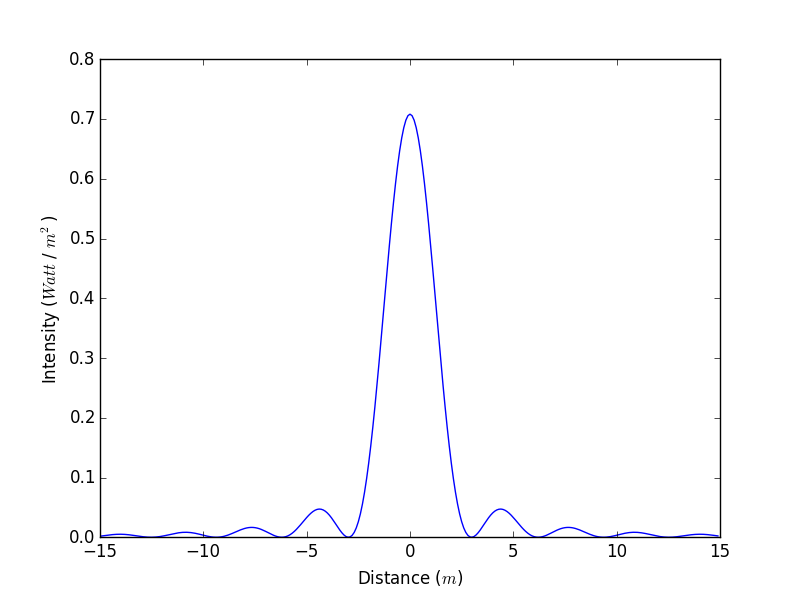
\includegraphics[scale=0.45]{figure_1.png}
\caption{Plot between distance and intensity}
\end{figure}

\begin{flushleft}
	As it should be, Intensity decreases by increasing the distance. Where at the position where source is placed we have high intensity peak.
\end{flushleft}
Next;\\
Plot between distance and intensity, for four antenna sources arrange in a linear array and by managing phase between them, we get interference pattern.
\begin{verbatim}
import numpy as np
import matplotlib.pyplot as plt
from math import sqrt, sin, pi

w=1.0
k=1.0
L=10.0 / k
P=0
# Calculate fringe spacing:
#d = 2 * 5           # Slit-spacing
#fs = 2 * pi * L / (k * d)

#print("Slit-spacing = {} produces fringe spacing = {}".format(d, fs))

ds = [-12, -4, 4, 12]
#sources=[(distance,phase)]
sources = [(-12, 0), (-4,0), (4,0), (12,0)]

def r(x,d):
return sqrt(L**2+(x-d)**2)

def Ex(x,d,p,t):
return ((x-d)/r(x,d)**2)*(sin(k*r(x,d)-w*t+p))

def Ey(x,d,p,t):
return (L/r(x,d)**2)*(sin(k*r(x,d)-w*t+p))

def I(x,sources,t):
Ox=0
Oy=0
for d, p in sources:
Ox+=Ex(x,d,p,t)
Oy+=Ey(x,d,p,t)

return Ox**2+Oy**2

def trapezoidal(f, a, b, n):
h = float(b - a) / n
s = 0.0
s += f(a)/2.0
for i in range(1, n):
s += f(a + i*h)
s += f(b)/2.0
return s * h

xs=[]
ys=[]

for x in np.linspace(-20,20,1000):
y = trapezoidal(lambda t: I(x,sources,t), -pi/w, pi/w, 100) / (2 * pi)

xs.append(x)
ys.append(y)

plt.plot(xs,ys)
plt.show()   
\end{verbatim}
\begin{figure}[ht]
	\centering	
    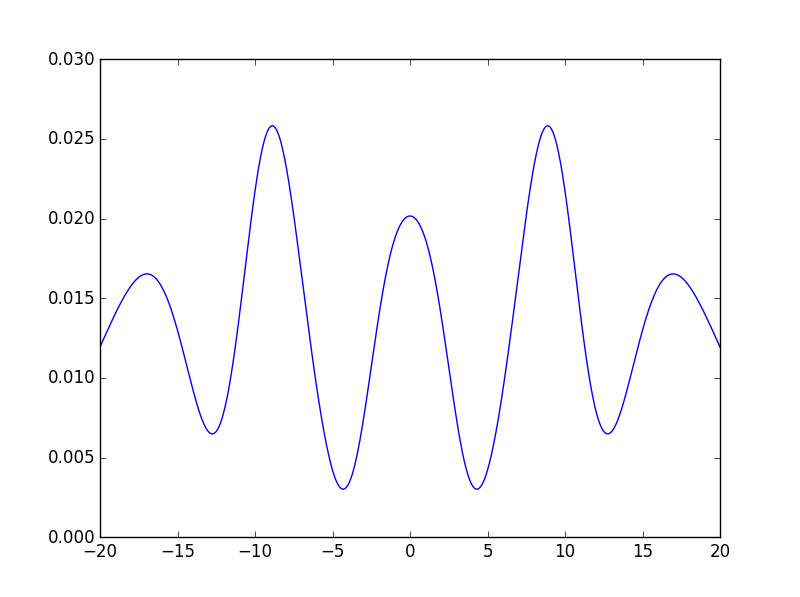
\includegraphics[scale=0.45]{figure_2.png}
	\caption{Plot between distance and intensity}
\end{figure}



%\end{document}
